\chapter{Design}

\section{Requirements}
In order to answer the research questions and produce public dataset at the end, the system should be capable to:
\begin{enumerate}
	\item Have a knowledge model describing how the data should be stored (in RDF format).
	\item Download LinkedIn personal public profiles and company public profiles, the data should be in HTML format.
	\item Extract data from the raw HTML files.
	\item Normalise the metadata to provide consistent and structure output, which means the system should be able to correct dirty data. This is important for upper layer, such as \gls{ui} that powered by SPARQL query, as minimum efforts are required if we have normalised data.
	\item Convert the data into RDF triples, and store it in a public accessible triplestore.
\end{enumerate}

Additionally, the system also have a number of non-functional requirements that need to be fulfilled:

\begin{description}
	\item \textbf{Crawling performance and parsing performance} \hfill \\
	The system should be able to download and parse enough profiles in a small number of days. Because timeliness is the nature of user generated content, if it takes too long to do this, we lost the chance of getting first hand information.
	\item Query performance \hfill \\
	The system should be able to respond to the query from user interface quickly enough to make sure the \gls{ui} usability.
	\item The choise of programming language(s) \hfill \\
	The ideal programming language(s) for this project should be dynamic typing, widely used, cross platform scripting language. The reason behind that is we want quickly iterate the program. As parsing and converting user generated content are hard, we cannot make assumptions about anything. Therefore, statically typed, compiled programming language (such as C++ and Java) is incapable for this task. Perl, Python are two possible options. But since Python is easy to learn and have rich communities support in terms of Semantic Web and Natural Language processing, we finally decide to use Python to implement our parse and RDF converter.
\end{description}


\section{Knowledge model}

As discussed in the previous chapter, we decide to use Semantic Web technologies for knowledge modelling. The first thing we need to do is the come out with an Ontology that can reflect the actual state of LinkedIn personal profile and company profile. After investigate with samples and discuss with the upper layer \acrshort{ui} designer, we come out with Figure~\ref{fig:KnowledgeModel}

\begin{figure}[H]
	\centering
	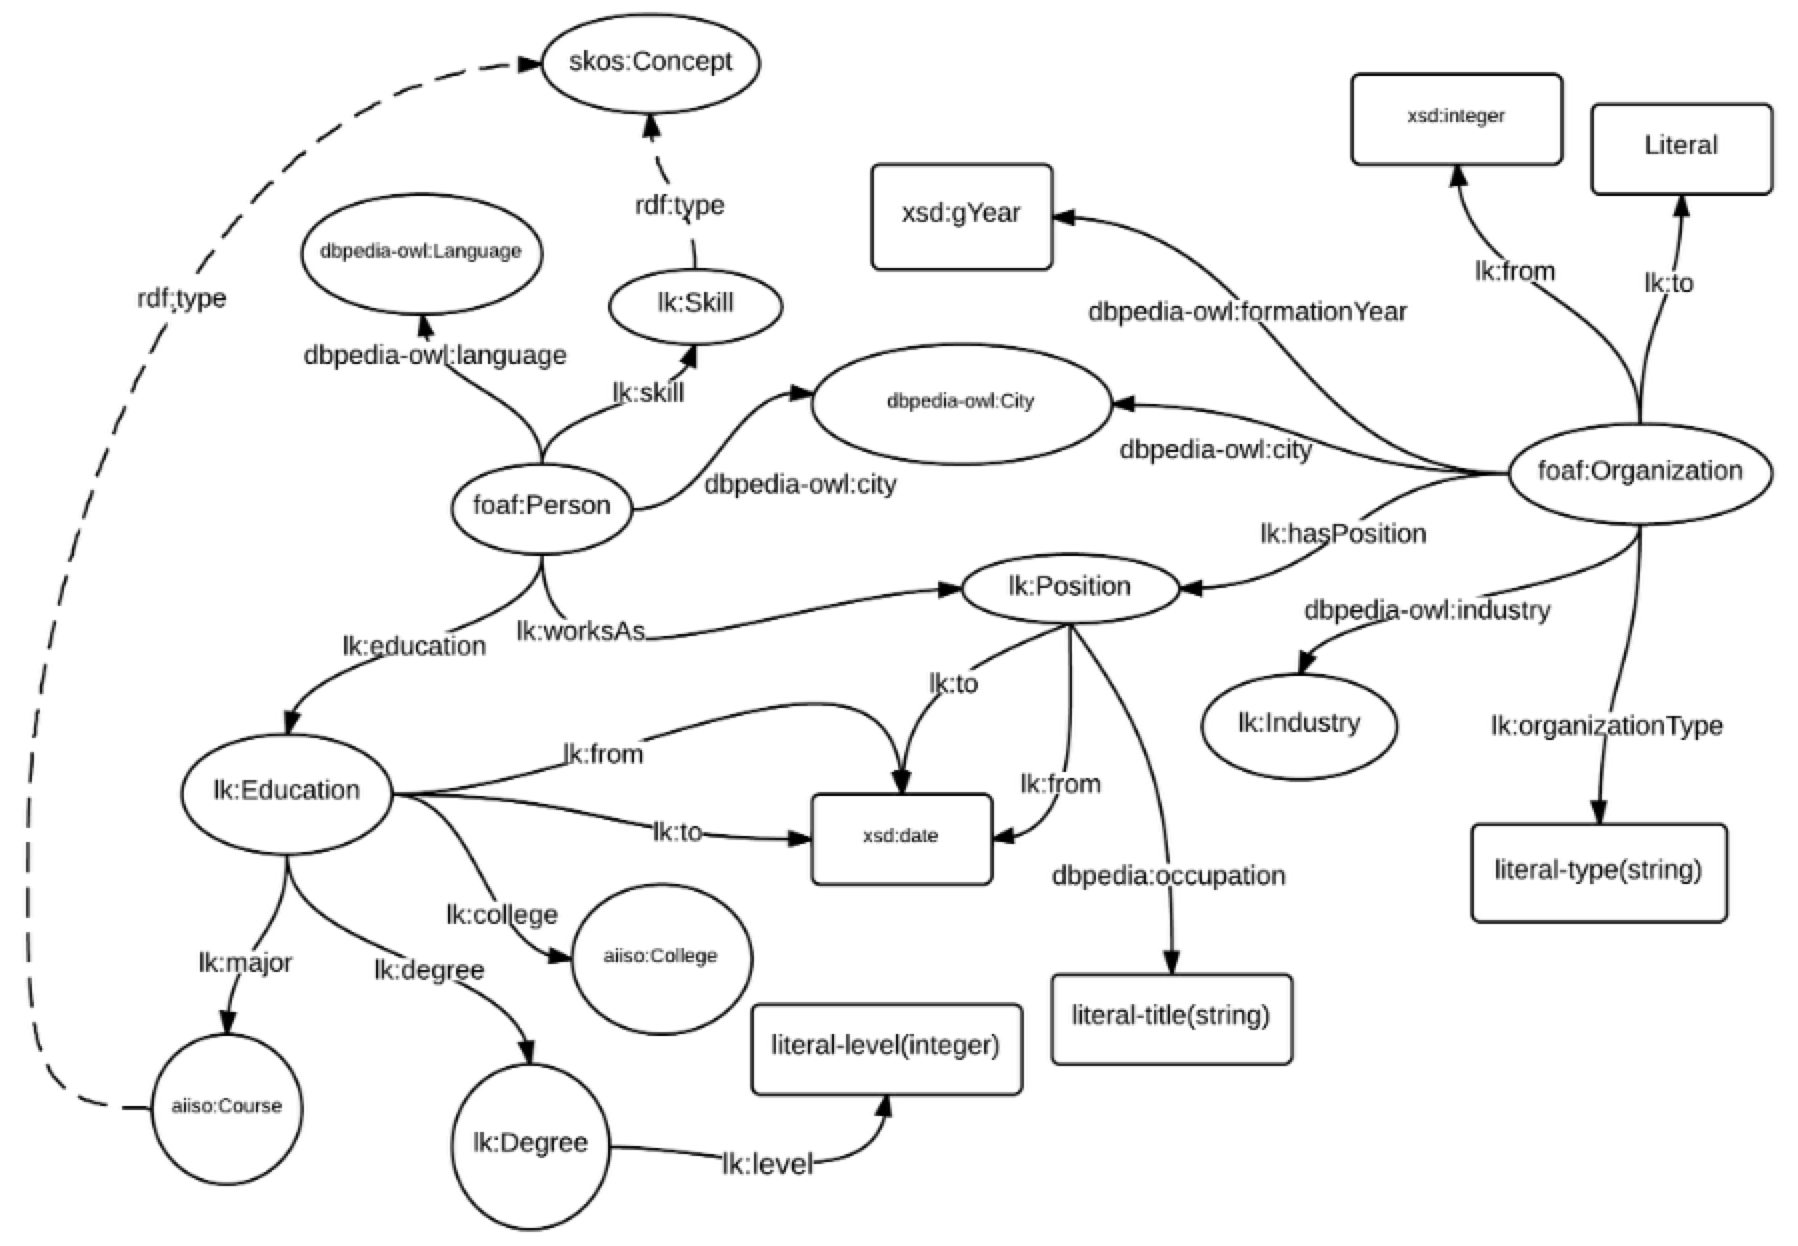
\includegraphics[width=1.0\textwidth]{images/knowledge-model.png}
	\caption{Knowledge Model for Linked public profile and company profile\protect}
	\label{fig:KnowledgeModel}
\end{figure}

As shown on the figure, the model can be divided into three cores: Person, Education and Organization. In LinkedIn personal profiles, a person might have currect living city, skills, work position, job title, start date and end date of the position. Besides, a person will have education background, such as college name, major, degree and start year and end year of the college.

For a LinkedIn company profile, it might have, headquarters, company type (public, private own, etc.) and industry type (e.g. \gls{it}) and company size.

Our knowledge model links the personal profile with company profile using ``position''. The whole graph is linked so that we can perform arbitrary query. For example, we can discover the relations between education background and organisation through person and position.

One key thing to note is Semantic Web is built around the idea of triples, which means an expression has the structure of ``subject'', ``predicate'' and ``object''. In the graph, the names in circle are ``Class'', the link between two ``Classes'' is call ``Property'' (predicate), it is used to link an instance of one Class to an instance of another Class.

\section{System architecture}

According the requirements, we design the system as Figure~\ref{fig:SystemArchitecture} shows:

\begin{figure}[H]
	\centering
	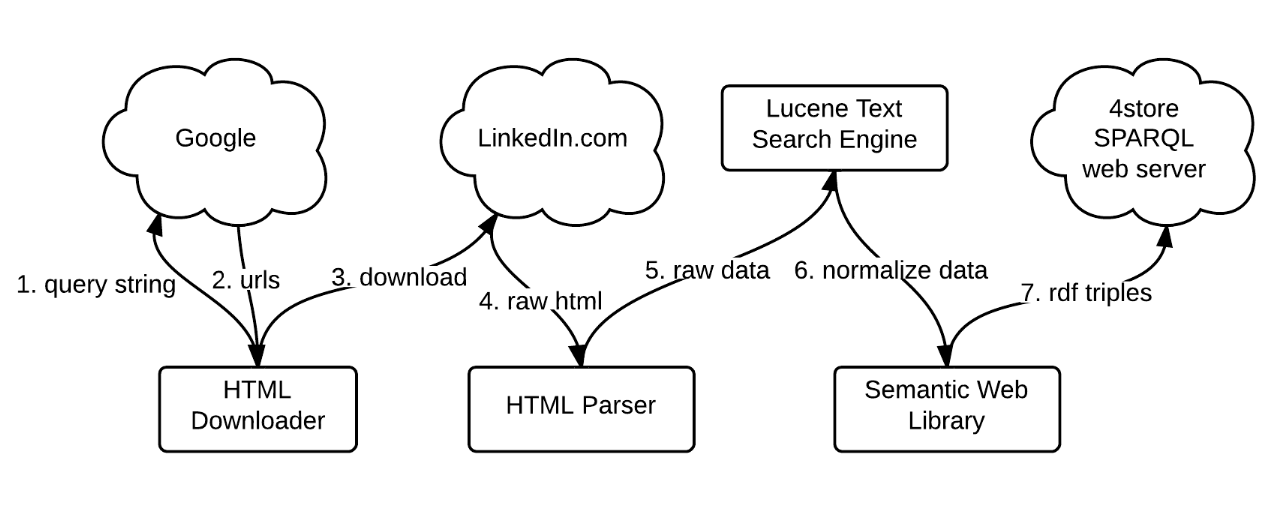
\includegraphics[width=1.0\textwidth]{images/system-architecture.png}
	\caption{System Architecture\protect}
	\label{fig:SystemArchitecture}
\end{figure}

\newacronym{api}{API}{Application programming interface}
\newacronym{url}{URL}{Uniform resource locator}

As LinkedIn.com will not provide \gls{api} for downloading their public profiles, we need to do it using Google search result.

So the system flow will be as follows, this description is a brief overview of the system process, more details will be given in the next chapter:
\begin{enumerate}
	\item Use Google search engine to query for profiles in LinkedIn Ireland.
	\item Get the response from Google, and download the html files base on the \gls{url} in response content.
	\item Call the parser to parse the HTML files and get the fields that will be used, as shown in the Figure~\ref{fig:KnowledgeModel}.
	\item Then the data extracted will be sent to a data normalisation module (Lucene search engine in this case), where the data will be cleaned up and normalised.
	\item Finally we can build the RDF triples using the normalised data and put them into our triplestore.
\end{enumerate}

\section{Design decisions}

There are several decisions we make to guarantee the final results come out smoothly.

Firstly, we decide to separate the profile downloader module with the profile parser module. It means we first run the module and download enough profiles, then we start to call parser module. The reason behind that is downloading profiles will consume a large amount of Google and LinkedIn resources, which implies that our connection can be switched off at any time by remote server. Therefore we don't want to do parsing together with downloading, since we don't want to spend extra effort in Network problem handing. Another point is that our final result will be in RDF format, hence if we do parsing together with downloading, extra storage and data structure is required to store this intermediate result.

Secondly, a simple database is required to keep track of which url is downloaded, which profile is parsed and had been converted into RDF format. Because we are handling a very large amount of profiles, and the correctness of the parse has to be adjusted during parsing, so it's unrealistic to assume that our program can parse and convert all the data with one-click. For example, if an unhandled exception occurred and stop the program, we can start parsing the remaining profiles if we have a database keeps track of the status.

Thirdly, just as the first reason we highlighted, the parser module, data normalisation module and RDF conversion module will form a pipeline. It means the output from previous module will be feed as input of the next module. The reason is, we don't have to store the intermediate result from the previous two modules.
